\section{The topologist's sine curve}
Because of \Cref{CauchyDfns} we can make the following definition:
\begin{definition}%[The topologist's sine curve]
  For $k:\mathbb N$, define $s_k:[\frac1k,1] \to [-1,1]$ by $s_k(x) = \sin(\frac1x)$ and $\mathcal S_k \subseteq [0,1] \times [-1,1]$ by 
  $$\mathcal S_k = ([0, \frac1k] \times [-1,1]) \cup graph(s_k)$$
  We define \textbf{the topologist's since curve} $\mathcal S = \bigcap_{k:\mathbb N} \mathcal S_k$. 
\begin{figure}[h!]
  \centering
  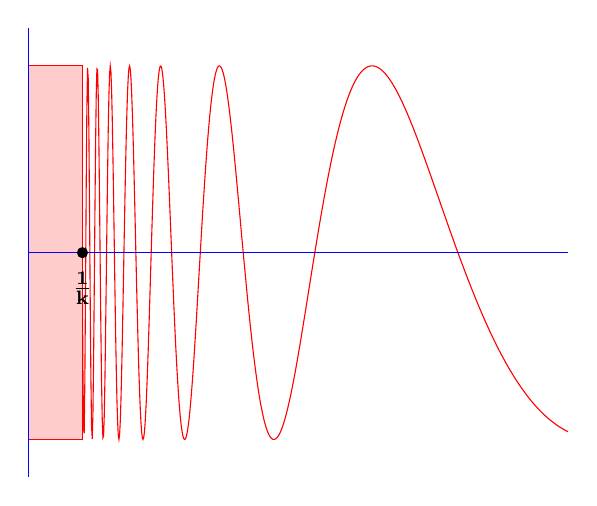
\begin{tikzpicture}
    \begin{axis}[axis lines=middle, xmin = 0 , ymin = -1.2 , ymax = 1.2 , xmax = 0.2, xtick=\empty, ytick=\empty, axis line style={color=blue, line width=0.6pt, -}, axis on top ]
      \addplot[domain=0.01:1, samples = 4000, color = red]{sin((deg(1/x)))};
      \addplot[draw=red, fill=red!20] coordinates {(0,-1) (0.02,-1) (0.02,1) (0,1)} \closedcycle ;
      \addplot[
  only marks,
  mark=*,
  mark size=1.8pt,
  color=black
] coordinates {(0.02,-0.00)};
\node[below] at (axis cs:0.02,-0.05) {$\mathbf{\frac1k}$};
    \end{axis}
  \end{tikzpicture}
  \caption{A picture of $\mathcal S_k$. The topologist's sine curve $\mathcal S$ is defined as the intersection of all such $\mathcal S_k$.}
\end{figure}

\end{definition}
  We shall denote $\iota_k : \mathcal S_k \to [0,1] \times [-1,1]$ 
  and $\iota:\mathcal S \to [0,1] \times [-1,1]$ for the inclusion maps, and $\pi_0:[0,1] \times[-1,1] \to [0,1],
\pi_1:[0,1] \times[-1,1] \to [-1,1]$ for the projection maps. 


\begin{lemma}
  The topologists's sine curve is a compact Hausdorff space.
\end{lemma}
\begin{proof}
  Note that both $[0,\frac1k] \times [-1,1]$ and $graph(s_k)$ are the image of compact Hausdorff spaces, hence closed by \Cref{CHausClosedImage}.
  By \Cref{ClosureClosedOpen} is follows that $\mathcal S$ is closed. We conclude by \Cref{CHausClosedImage}
\end{proof}

%\begin{remark}\label{NonZeroOnGraph}
%  Let $(x,y):[0,1]\times[-1,1]$. By \Cref{positiveNumbersCharacter}, if $(x,y)\in \mathcal S$ and $x \neq 0$, there is some $k:\N$ such that $x>\frac1k$ and hence $(x,y)\in \mathcal S_k$. 
%\end{remark}

%\begin{corollary}\label{NonZeroOnGraph}
%  By the above, if for some $x:[0,1] \times [-1,1]$ we have $x\in \mathcal S$ and $\pi_1(x)\neq 0$, there must be some $k\in\mathbb N$ with $x \in graph(t_k)$ and hence $\pi_2(x) =\sin(\frac1{\pi_1(x)})$. 
%\end{corollary}

\subsection{The curve is not path-connected}
\begin{remark}\label{topbottomSeq}
  For each $k:\N$, denote $t_k = \frac1{(2k+\frac12) \pi}$ and  $b_k = \frac1{(2k+\frac32) \pi}$. 
  Note that for all $k:\N$ we have $\sin(\frac1{b_k})=-1, \sin(\frac1{t_k})=1$ and
  $1>t_k>b_k>t_{k+1}>b_{k+1}>0$. 
\end{remark}
\begin{lemma}\label{cofinaltbseq}
  Given $r:[0,1]$ with $r>0$, there exists some $k:\N$ with $t_k,b_k<r$.  
\end{lemma}
\begin{proof}
  By \Cref{positiveNumbersCharacter}, there is some $k:\N$ with $\frac1k<r$. As $(2k+\frac32)\pi,(2k+\frac12)\pi>k$, this $k$ suffices.
\end{proof}
\begin{lemma}\label{NonZeroOnGraph}
  Let $(x,y):[0,1]\times[-1,1]$ be such that $(x,y)\in\mathcal S$ and $x>0$.
  Then $y = \sin(\frac1x)$
\end{lemma}
\begin{proof}
  By \Cref{positiveNumbersCharacter}, there is some $k:\N$ such that $x>\frac1k$ and hence $(x,y)\in \mathcal S_k$ and $y = \sin(\frac1x)$. 
\end{proof}

\begin{lemma}\label{SineWillHitTopBot}
  Let $\gamma:[0,1] \to \mathcal S$. 
  Assume that $\pi_1(\gamma(0)) = 0$ and $\pi_1(\gamma(r))>0$ for some $r:[0,1]$. 
  Then there exist some $u,v:[0,1]$ with $0<u<v<r$ such that $\pi_2(\gamma(u)) = 1$, and $\pi_2(\gamma(v)) = -1$. 
\end{lemma}
\begin{proof}
  By \Cref{cofinaltbseq}, there exists some $k:\N$ such that $0 < b_k<r$. 
  We can thus apply \Cref{IntermediateValue} to $\pi_1\circ \gamma : [0,1] \to [0,1]$ to find some $v:[0,1]$ with $\pi_1(\gamma(v)) = b_k$. Then by \Cref{NonZeroOnGraph} and \Cref{topbottomSeq} we find that $\pi_2(\gamma(v)) = -1$. 
  The case for $u$ is similar. 
\end{proof}

\begin{theorem}[The topologist's sine curve is not path-connected]
  There is no map $\gamma:[0,1] \to \mathcal S$ such that $\gamma(0) = (0,0)$ and $\gamma(1) = (1,sin(1))$. 
\end{theorem}
\begin{proof}
  By applying dependent choice to \Cref{SineWillHitTopBot}, 
  we can find sequences $u_i,v_i,~i:\N$ such that $\pi_2(\gamma(u_i)) = 1, \pi_2(\gamma(v_i)) = -1$ and 
  $u_{i+1}<v_{i+1}<u_i<v_i$ for all $i:\mathbb N$. 
  We now apply \Cref{UniformContinuity} for $\epsilon =2 $.
  There is some $\delta>0$ such that $d(u_i, v_j)\geq \delta$ for any $i,j:\mathbb N$ as  $d(\gamma(u_i), \gamma(v_j)) \geq 2$. 
  Therefore, the sequence $u_i$ is decreasing with steps of at least size $2\delta>0$. 
  But this means that for $N>\frac1{2\delta}$, we have $u_{N}<0$, while $u_N :[0,1]$, which is a contradiction. 
\end{proof}

\begin{remark}
  One could define an equivalence relation on any type $X$ such that 
  $x\sim y$ iff there is a path from $x$ to $y$. 
  The equivalence classes of this relation would normally be called the path-connected components. 
  We conjecture that the space of path-connected components of $\mathcal S$ is equivalent to the type of open propositions. 
\end{remark}

\subsection{The shape of the curve}
We will prove that $\mathcal S$ is $[0,1]$-contractible. 
\begin{remark}
  We denote for each $r:[0,1]$ the fiber 
  $\mathcal S_r:= (\pi_1\circ \iota)^{-r}$. 
  Note that 
  $\mathcal S_r = \mathcal S \cap (\pi_1^{-1}(r)) = 
  \mathcal S \cap (\{r\} \times [-1,1])$, and that $\mathcal S_r$ is closed for all $r:[0,1]$. 
\end{remark}


\begin{lemma}\label{fiberInhabited}
  $\pi_1\circ \iota : \mathcal S \to [0,1]$ is surjective.  
\end{lemma}
\begin{proof}
  We shall show that for each $r:[0,1]$ the fiber $\mathcal S_r$ is merely inhabited. 
%
  By \Cref{compactnessCHaus}, 
  it's sufficient to show that $\pi_1^{-1}(r) \cap \mathcal S_k$ 
  is merely inhabited for any $k:\mathbb N$. 
%
  Let $k:\mathbb N$. 
  As we're showing a proposition, we make for each $k:\N$ a case distinction based on \Cref{LLPO}:
%  Note that $r\leq \frac1k \vee r \geq \frac 1k$. 
  \begin{itemize}
    \item If $r\leq \frac1k$, we have that $(r,0) \in \mathcal S_k$. 
    \item If $r\geq \frac1k$, $\frac1r$ is well-defined and 
      $(r,\sin(\frac1r)) \in \mathcal S_k$. 
  \end{itemize}
  Hence in both cases we have that $\pi_1^{-1}(r) \cap \mathcal S_k$ is inhabited, as required. 
\end{proof}

\begin{lemma}
  For each $k:\mathbb N$ and $r:[0,1]$, $\mathcal S_k\cap \pi_1^{-1}(r)$ is convex. 
\end{lemma}
\begin{proof}
  Suppose that $(x,y), (x',y')$ both lie in $\mathcal S_k\cap \pi_1^{-1}(r)$. 
  Suppose furthermore that $\alpha,\beta:[0,1], \alpha+ \beta = 1$. 
  We will show that $\alpha\cdot (x,y) + \beta\cdot (x',y') $ also lies in 
  $\mathcal S_k \cap \pi_1^{-1}(r)$. 

  Recall that 
  $\mathcal S_k = [0,\frac1k] \times [-1,1]  \cup graph(s_k)$. 
  As we will show a proposition, we can make a case distinction 
  for both $(x,y), (x',y')$ on whether they come from $[0,\frac 1k] \times [-1,1]$ or 
  from $graph(s_k)$.
  \begin{itemize}
    \item 
      If either comes from $[0,\frac1k] \times [-1,1]$, we must have that 
      then $r \leq \frac1k$. 
      Then $\pi_1^{-1}(r) = \{r\} \times [-1,1]\subseteq \mathcal S_k$. 
      It follows that $\pi_1^{-1}(r) \cap \mathcal S_k = \{r\} \times [-1, 1]$, which is convex. 
    \item 
      If both come from $graph(t)$, 
      then $x = x' = r$ and $y = y' = \sin(\frac1r)$. 
      Hence $(x,y) = (x',y')$ and thus $\alpha(x,y) + \beta(x',y') = (x',y')$. 
  \end{itemize}
  In both cases we conclude that $\alpha (x,y) + \beta(x',y')$ lies in 
  $\mathcal S_k\cap \pi_1^{-1}(r)$. 
\end{proof}

\begin{corollary}\label{fiberConvex}
  For each $r:[0,1]$, the fiber 
  $\mathcal S_r$ is convex. 
\end{corollary}
\begin{proof}
  Any intersection of convex subspaces of $\mathbb R^n$ is itself convex
\end{proof}
\begin{theorem}
  $\mathcal S$ is $[0,1]$-contractible. 
\end{theorem}
\begin{proof}
%  We write $\mathcal S = \sum\limits_{r:[0,1]} \mathcal S_r$.
  By \Cref{fiberConvex} and \Cref{fiberInhabited}, each fiber $S_r$ is convex and inhabited, hence by \Cref{ConvexInhabitedToContractible} also $[0,1]$-contractible. 
%
  Thus both the maps $\pi_0 \circ i :\mathcal S \to [0,1]$ and $[0,1] \to 1$ have $[0,1]$-contractible fibers. 
  By \parencite[Lemma 1.33]{modalities}, so does their composite. 
  It follows that $\mathcal S$ is $[0,1]$-contractible. 
\end{proof}
